\section{Progettazione Concettuale}
Questa fase è di cruciale importanza poiché definisce il contenuto informativo del data mart. Tutta la prima parte di questa fase si occupa di capire qual è il modello che viene utilizzato, quindi individuare i vari costrutti che si potranno utilizzare. Non vi è uno standard ufficiale per la realizzazione della parte di progettazione concettuale del data mart. È possibile utilizzare il modello E-R per il data mart? No, perché è troppo espressivo e perché è nato per modellare realtà di business fatte in qualunque modo. Qui il modello deve essere multidimensionale e bisogna rispettare dei vincoli; quindi, ci devono essere gerarchie progettate in un certo modo. Molti progettisti disegnano direttamente gli schemi a stella (schemi logici relazionali). Questo tipo di approccio non è conveniente e funziona male perché racchiude solo la definizione di un insieme di relazioni e di vincoli di integrità (sono denormalizzate in pratica). 

Il formalismo che bisogna utilizzare si chiama \textbf{Dimensional Fact Model (DFM}). Ha una larga diffusione nei contesti italiani ed esteri, ma soprattutto nel mondo della ricerca. È un modello concettuale grafico pensato per:
\begin{itemize}
	\item 
	Supportare efficacemente il progetto concettuale
	\item 
	Permette di verificare che le interrogazioni (query OLAP) siano effettivamente esprimibili sul cubo che stiamo disegnando 
	\item 
	Supportare un dialogo tra progettista e utente finale
	\item 
	È fondamentale per la documentazione che deve essere espressiva e non ambigua
	\item 
	Creare una piattaforma stabile da cui partire per il progetto logico
\end{itemize}

Quando si utilizza il \textbf{DFM} creiamo degli schemi detti schemi di fatto. Trattandosi di schemi multidimensionali, ovviamente, disegneremo fatti, misure e gerarchie. Distingueremo la parte del DFM in costrutti di base e costrutti avanzati. I primi coprono un pò di più dell’espressività del modello multidimensionale. I secondi, invece, servono per modellare le sfumature che si incontrano nei progetti reali. 
\subsection{I costrutti di base}
\begin{itemize}
	\item
	\textbf{Fatto}: è un fenomeno di business che accade dinamicamente all’interno dell’azienda. È essenziale che un fatto abbia aspetti dinamici, ovvero evolva nel tempo
	\item 
	\textbf{Dimensione}: attributi numerici che quantificano il fatto da un certo punto di vista (il voto di laurea, qtà acquistata)
	\item 
	\textbf{Misura}: coordinate di accesso al cubo. 
\end{itemize}
\begin{figure}[H]
	\centering
	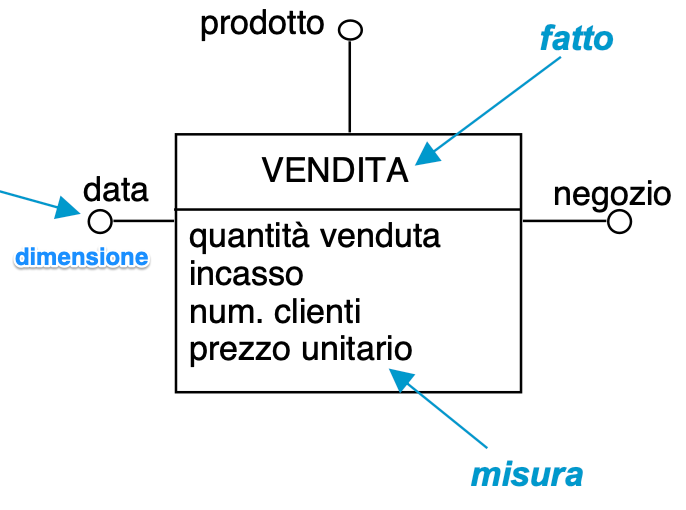
\includegraphics[width=0.7\linewidth]{img/example_fatto}
	\caption{Esempio di ...}
	\label{fig:exfatto}
\end{figure}
Quindi il tipo di relazione che ho tra prodotto, data e negozio è una classica associazione molti a molti. Dunque, un \textbf{fatto} esprime una associazione molti a molti tra le dimensioni.

Una \textbf{gerarchia} è una sequenza di attributi collegati tra di loro da associazioni molti ad uno, ossia da dipendenze funzionali. Le gerarchie non sono necessariamente dei percorsi, ma possono avere forme più complesse. In particolare possono essere degli alberi, i cui nodi si chiamano attributi dimensionali, i quali descrivono le dimensioni in modo via via più aggregato. L’\textbf{albero} non orientato è un grafo aciclico. In quest' albero la radice è la dimensione, mentre gli archi rappresentano dipendenze funzionali. 

Un \textbf{evento primario} è una particolare occorrenza di un fatto, individuata da una ennupla costituita da un valore per ciascuna dimensione. A ciascun evento primario è associato un valore per ciascuna misura. Per modellare il concetto dell’aggregazione sul DFM si ragiona in termini di group-by-set (livello di aggregazione) e di conseguenza aggrego (la sparsità diminuisce) nella query gli eventi primari in eventi secondari. Tanti eventi primari contribuiscono a costruire un evento secondario.  

Dato un DFM qualsiasi, in qualunque modo si scelga un sottoinsieme di attributi dimensionali, a patto che non ci siano dipendenze funzionali, ho un possibile group-by-set. 

\subsection{I costrutti avanzati}
\begin{itemize}
	\item 
	\textbf{Attributo descrittivo}: aggiunge delle informazioni su un attributo dimensionale, a cui è connesso da una associazione uno-a-uno. Questo tipo di attributi possono essere utilizzati per la selezione ma non possono essere utilizzati per l’aggregazione (non possono finire dentro ad un group-by-set). Gli attributi descrittivi non hanno figli. Posso discretizzare gli attributi descrittivi trasformandoli in un attributo dimensionale.  
	\item 
	\textbf{Archi opzionali}: è un arco molti-ad-uno ma entra in gioco la cardinalità minima. Con l’arco opzionale dico che per alcuni valori del padre non è definito nessun valore del figlio. 
		\begin{figure}[H]
		\centering
		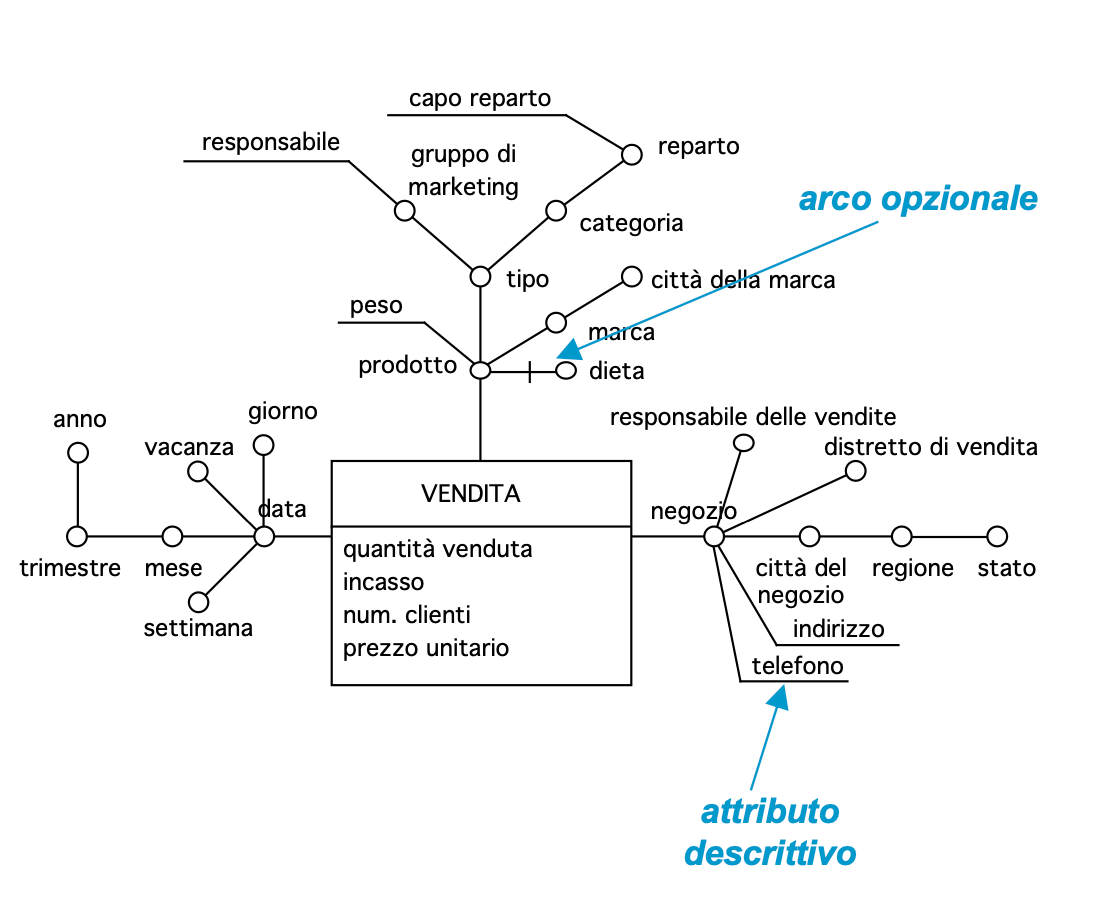
\includegraphics[width=0.6\linewidth]{img/descrittivo}
		\caption{Attributo descrittivo e arco opzionale}
		\label{fig:descr}
	\end{figure}
	\item 
	\textbf{Gerarchia condivisa}: in realtà le gerarchie possono avere dei cicli. Ho quattro modi per creare dei cicli nelle gerarchie del DFM, con quattro significati diversi. Il primo modo è la gerarchia condivisa, che è quello più debole, perché non pone vincoli sulle istanze. Una gerarchia condivisa è un albero che viene usato due o più volte all’interno dello stesso schema di fatto.
	\begin{figure}[H]
		\centering
		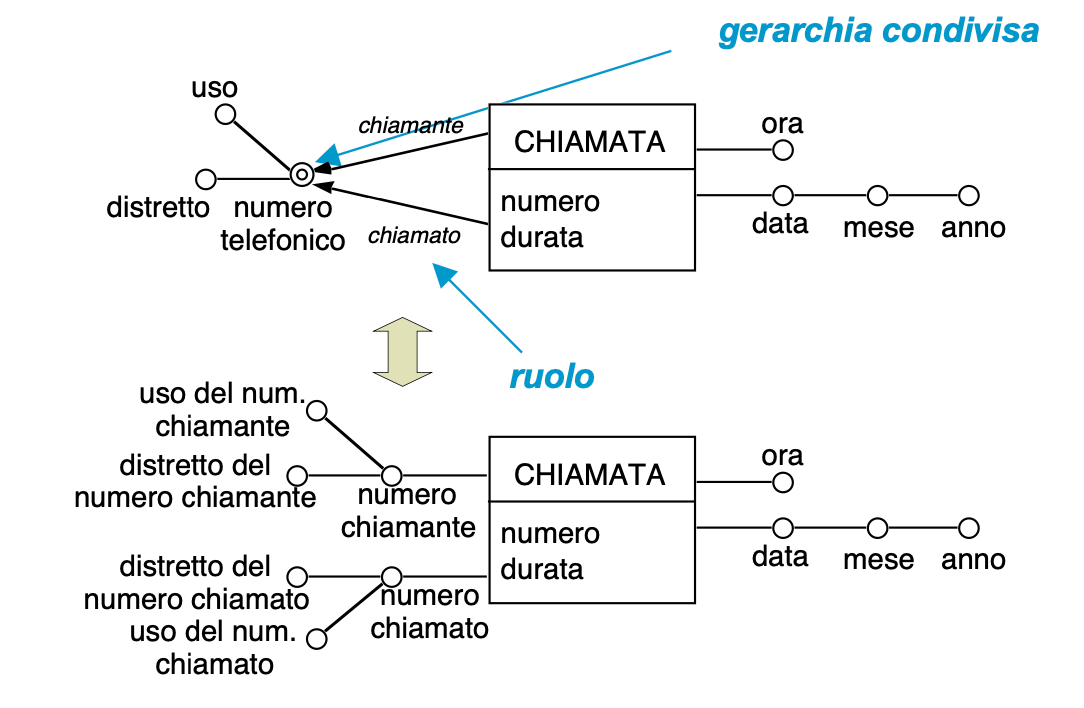
\includegraphics[width=0.6\linewidth]{img/condivisa}
		\caption{Gerarchia condivisa}
		\label{fig:condivisa}
	\end{figure}
	\item 
	\textbf{Convergenza}: aggiungo un vincolo sulle istanze. Mentre nel caso della condivisione non pongo vincoli sulle istanze, nel caso della convergenza non solo ho più percorsi che partono da un punto e arrivano nell’altro punto, ma qualunque dei due percorsi io prenda per ogni valore del punto di partenza arrivo sempre nello stesso punto di arrivo. Ho un vincolo aggiuntivo sulle istanze. 
	\begin{figure}[H]
		\centering
		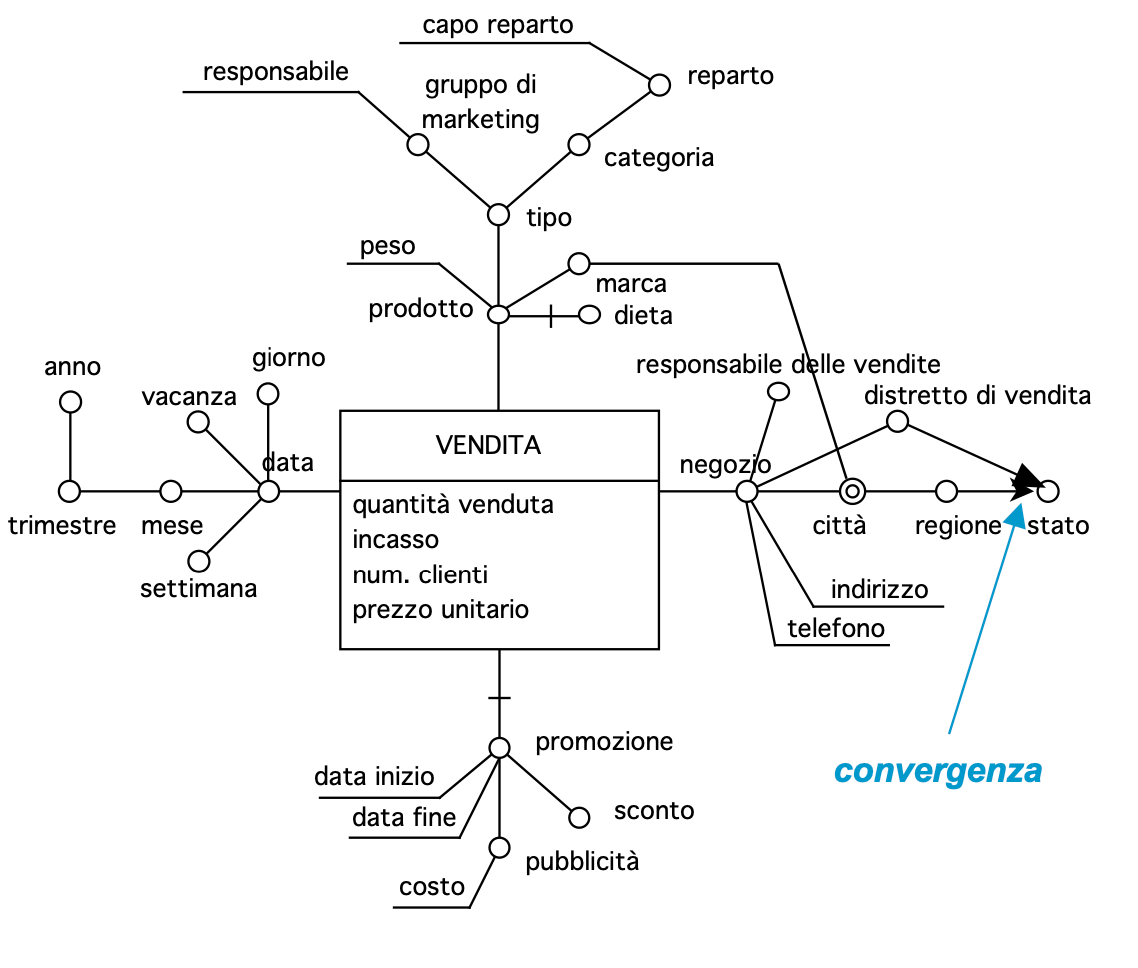
\includegraphics[width=0.6\linewidth]{img/convergenza}
		\caption{Convergenza}
		\label{fig:conv}
	\end{figure}
	\item 
	\textbf{Gerarchia incompleta}: per alcune istanze della gerarchia mancano dei valori di alcuni valori intermedi. La particolarità della gerarchia incompleta è che si hanno per le diverse istanze della gerarchia, un numero variabili di livelli pieni. 
		\begin{figure}[H]
		\centering
		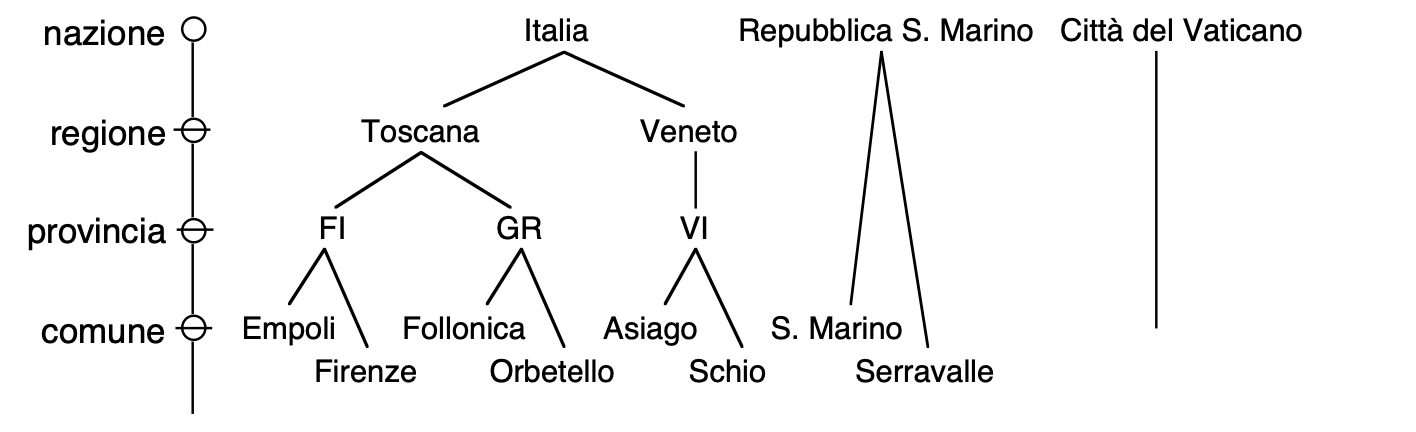
\includegraphics[width=0.7\linewidth]{img/incompleta}
		\caption{Gerarchia incompleta}
		\label{fig:incompleta}
	\end{figure}
	\item 
	\textbf{Additività}: esprime in che modo le misure possono essere aggregate. Di per sé le misure sono classificabili in tre categorie:
	\begin{itemize}
		\item 
		\textbf{Misure di flusso}: si riferiscono ad un periodo di tempo e vengono istanziate in modo cumulativo (il numero di prodotti venduti in un giorno, l’incasso mensile, il numero di nati in un anno). Sono quelle più semplice da gestire perché sono additive lungo tutte le dimensioni.
		\item 
		\textbf{Misure di livello}: vengono valutate in istanti di tempo (il numero di prodotti in inventario, il numero di abitanti di una città)
		\item 
		\textbf{Misure unitarie}: vengono valutate in particolari istanti di tempo, ma sono espresse in termini relativi (il prezzo unitario di un prodotto, la percentuale di scoto, il cambio di una valuta) 
	\end{itemize}
	
	
	La misura è detta \textbf{additiva} lungo una dimensione se i suoi valori possono essere aggregati lungo la corrispondente gerarchia tramite l’operatore di somma, altrimenti è detta non-additiva. Una misura \textbf{non-additiva} è non-aggregabile se nessun operatore di aggregazione può essere usato su di essa.  
	
	Uno schema di fatto si dice \textbf{vuoto} se non ha misure. In questo caso, il fatto registra solo il verificarsi di un evento.
\end{itemize}
	
	\subsection{Editing dell'albero}
	 Ci si accorge che alcuni attributi dell’albero non sono d’interesse per l’analisi. L’eliminazione del nodo si può fare in due modi:
	 \begin{itemize}
	 	\item 
	 	\textbf{Potatura}: taglio quel nodo e tutti i suoi figli
	 	\item 
	 	\textbf{Innesto}: si elimina un nodo mantenendo i suoi figli
	\end{itemize}
	 L’innesto deriva dalla teoria delle dipendenze funzionali. Quando un \textbf{vertice opzionale} viene innestato, tutti i suoi figli ereditano il trattino di opzionalità. Nel caso di potatura o innesto di un vertice opzionale v con padre "v’" è possibile aggiungere a "v’" un nuovo figlio "b" corrispondente a un attributo booleano che esprima l’opzionalità. 
	 
	 Tutte le volte  che durante l’editing si decida di eliminare un attributo che è un figlio diretto della radice e fa parte della chiave della relazione che si è scelto come fatto oppure fa parte dell’identificatore dell’entità che si è scelto come fatto si sta cambiando la granularità. 
	 
	 Nella pratica possono rendersi necessarie ulteriori manipolazioni sull’albero degli attributi:
	 \begin{itemize}
	 	\item
	 	può essere necessario modificarne radicalmente la struttura sostituendo il padre di un certo nodo: ciò corrisponde ad aggiungere o eliminare una dipendenza funzionale. 
	 	\begin{figure}[H]
			\centering
			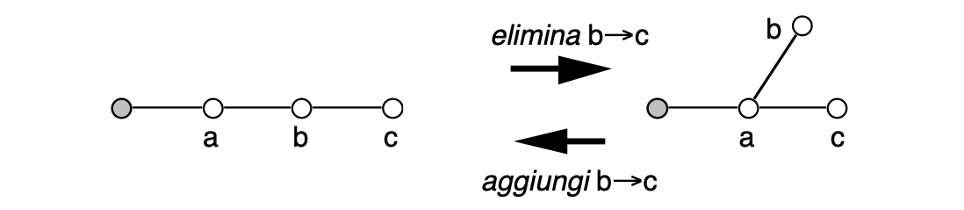
\includegraphics[width=0.6\linewidth]{img/editing}
			\caption{Editing dell'albero}
			\label{fig:editing}
	 	\end{figure}
 	Perché dovrei aggiungere o togliere una dipendenza funzionale? Aggiungere una dipendenza funzionale conviene se lo schema sorgente non è perfettamente normalizzato.
 	
 	A volte ci capiterà di eliminare delle dipendenze funzionali. L’unico caso è quando dobbiamo scegliere come misura un attributo che non è figlio diretto della radice. 
	 	\item 
	 	può capitare che dentro l’albero ci finiscano degli archi che rappresentano dei casi particolari di associazioni molti a uno, ovvero associazioni uno-a-uno. Questo può succedere in più situazioni: se partiamo da un E/R in cui abbiamo gerarchie di specializzazione, la gerarchia da luogo ad associazioni binarie uno-a-uno. Nell’E/R di partenza può capitare che si abbia già un’associazione uno-a-uno (esempio iscritto e tessera in palestra). Dentro il DFM non si possono avere archi tra due attributi dimensionali che rappresentano associazioni uno-a-uno, ma sempre molti-a-uno. 
	 	
	 	In presenza di un’associazione uno-a-uno vi sono due soluzioni:
	 	\begin{itemize}
	 		\item 
	 		quando il vertice v determinato dall’associazione uno-a-uno ha dei discendenti di interesse lo si può eliminare dall’albero tramite innesto
	 		\item 
	 		quando v non ha discendenti di interesse lo si può rappresentare come attributo descrittivo
	 		\item 
	 		in alcuni casi può convenire invertire i due nodi coinvolti
	 	\end{itemize}

	 \end{itemize}
 
 \subsection{Scelta delle dimensioni}
 Le \textbf{dimensioni} vanno scelte tra i figli diretti della radice e devono corrispondere ad attributi che abbiano un dominio finito e discreto. La loro scelta è cruciale per il progetto poiché definisce la granularità degli eventi primari. 
\subsection{Scelta delle misure}
Le \textbf{misure} sono i figli diretti della radice che non abbiamo scelto come dimensioni. Sono sempre attributi numerici (reali o interi). 
\subsection{Creazione dello schema di fatto} 
L’albero degli attributi può essere tradotto in uno schema di fatto che include le dimensioni e misure definite:
\begin{itemize}
	\item 
	le gerarchie corrispondono ai sottoalberi dell’albero degli attributi con radice nelle diverse dimensioni
	\item 
	il nome del fatto corrisponde al nome dell’entità scelta come fatto
	\item 
	è possibile potare e innestare l’albero per eliminare dettagli inutili
	\item 
	è possibile aggiungere attributi dimensionali definendo opportuni intervalli per attributi numerici
	\item 
	gli attributi che non verranno usati per l’aggregazione possono essere contrassegnati come descrittivi; tra questi compariranno in genere anche gli attributi determinati da associazioni uno-a-uno e privi di discendenti
	\item 
	per quanto riguarda eventuali attributi alfanumerici figli della radice ma non prescelti né come dimensioni né come misure:
	\begin{itemize}
		\item 
		se la granularità degli eventi primari coincide con quella dell’entità F, essi possono essere rappresentati come attributi descrittivi associati direttamente al fatto, di cui descriveranno ciascuna occorrenza
		\item 
		se invece le due granularità sono differenti, essi devono necessariamente essere potati
	\end{itemize}
\subsection{Carico di lavoro e volume dati}
Per il data mart si hanno diversi schemi di fatto che mostrano il contenuto informativo del data mart dal punto di vista concettuale indipendente dall’implementazione. Il prossimo passo sarà tradurre gli schemi concettuali in schemi logici (ROLAP). È opportuno fare un ragionamento sul carico di lavoro e volume dati. Il carico di lavoro indica le query che più frequentemente verranno sottoposte al sistema. Per definizione il carico di lavoro OLAP è estemporaneo, ma il nucleo del carico di lavoro si può prevedere. La query OLAP standard ha una clausola di group-by, richiede una o più misure, e ha delle clausole di selezione. 

Quindi durante questa fase inizio a organizzare tutte le query che ho catturato nell'analisi dei requisiti, verificano che siano supportati dagli schemi concettuali che ho disegnato e comincio a legarle agli utenti. Per gestire la variabilità del carico di lavoro bisogna fare un monitoraggio costante. Non tutte le query possono essere lanciate da tutti gli utenti, quindi si comincia con la \textbf{profilazione}, ovvero capire quali saranno i principali profili di utenti che dovranno accedere al data mart. Comincio con il legare quindi a ciascun utente delle aree di analisi che potrebbero essere utili. Devo spiegare per tutti gli utenti di ciascun profilo quali query potranno formulare. In questa fase è importante anche cominciare a misurare il volume dati. Misurare il volume dati significa per ciascun attributo che si ha nella gerarchia capire qual è la sua cardinalità di dominio. 

\end{itemize}

